\section{Spørgsmål 1}

\subsection{Fokuspunkter}
\begin{itemize}
	\item Forklar principperne bag Entity/Relationship modellering.
	\begin{itemize}
		\item Herunder princippet for et Entity Relationsship Diagram (ERD)
	\end{itemize}
	\item Hvorledes opstilles et ER Diagram?
\end{itemize}

\subsection{Litteratur}
\begin{itemize}
	
	\item Fra teori: Database Modeling and Design. Logical Design 5'th Ed.
	\begin{itemize}
		\item Ch. 1 (p1 - 11)
		\item Ch. 2 (p13 - 34)
		\item Ch. 3 (p35 - 53)
		\item Ch. 4 (p55 - 84)
	\end{itemize}
	
	\item Fra Database eLearning: \url{http://db.grussell.org/index.html}.
	\begin{itemize}
		\item Database Analysis and ER Modelling.
		\begin{itemize}
			\item Database Analysis.
			\item Entity Relationship Modelling - 2.
			\item Advanced ER Mapping.
		\end{itemize}
	\end{itemize}
	
%	\item Fra wikipedia:
%	\begin{itemize}
%		\item 
%	\end{itemize}
%	
%	\item Fra Agile Data Home Page:
%	\begin{itemize}
%		\item 
%	\end{itemize}
\end{itemize}

\newpage

% must
\subsection{Forklar pincipperne bag Entity/Relationship modellering}

Generelt bruges \textit{Three-Level Database Model}. Denne anvendes når et design og fysisk implementering af databasen skal laves, ud fra nogle bestemte krav. 

\begin{enumerate}
	\item \textbf{Conceptual Data Model}\\
	Sparsom på detaljer. Giver overblik og ikke-teknisk-personale kan læse den.
	\item \textbf{Logical Data Model}\\
	Indeholder detaljer om Entities (tabeller) og Relationships (keys).
	\item \textbf{Physical Data Model}\\
	Er detaljeret nok til at databasen kan laves udfra denne. Indeholder information om tabeller, kolonner, keys, data-typer, validation rules, database triggers, stored procedures, domains\footnote{Rækker? Attributter?}, and access constraints\footnote{Woot?}.
\end{enumerate}

Ud fra dette skema den fysiske database genereres.

% must
\subsection{Forklar princippet for et Entity Relationsship Diagram (ERD)}

Et ER-diagram bruger til at gengive \textit{real world} attributter. Vil typisk bestå af følgende:\\

\begin{figure}[h]
	\centering
	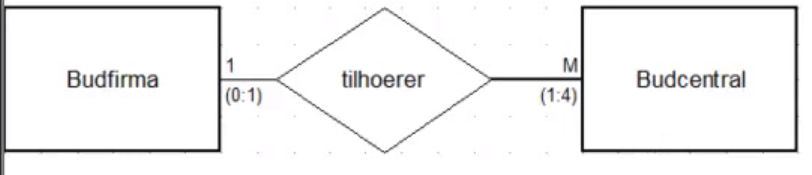
\includegraphics[width=0.83\linewidth]{figs/spm1/entity_in_relation}
	\caption{Eksempel på et ERD diagram.}
	\label{fig:erd}
\end{figure}

\subsubsection{Entity}

An entity is a thing that exists either physically or logically. An entity may be a physical object such as a house or a car (they exist physically), an event such as a house sale or a car service, or a concept such as a customer transaction or order (they exist logically—as a concept).

\subsubsection{Relation}
A relationship captures how entities are related to one another. Relationships can be thought of as verbs, linking two or more nouns. Examples: an owns relationship between a company and a computer, a supervises relationship between an employee and a department, a performs relationship between an artist and a song, a proves relationship between a mathematician and a conjecture.

\subsubsection{Attributter}
Entities and relationships can both have attributes. Examples: an employee entity might have a Social Security Number (SSN) attribute; the proved relationship may have a date attribute.

\subsubsection{Keys}

For mere om nøgler se side~\pageref{sec:keys}.

\paragraph{Primærnøgle}
\paragraph{Sekundærnøgle}

% must
\subsection{Hvorledes opstilles et ER Diagram?}




























